\documentclass[a4paper, 12pt]{article}
\usepackage[english]{babel}
\usepackage[utf8]{inputenc}
\usepackage[T1]{fontenc}
\usepackage{lmodern}
\usepackage{hyperref}
\usepackage[numbers, sort&compress]{natbib}
\usepackage{calc}
\usepackage{fancyhdr}
\usepackage{graphics}
\usepackage{nowidow}
\usepackage{color}
\usepackage{subcaption}
\usepackage{epsfig}
\usepackage{epstopdf}
\usepackage{verbatim}


\newlength{\oneLine}
\newlength{\halfLine}
\setlength{\oneLine}{12pt}
\setlength{\halfLine}{6pt}

\newlength{\eqMargin}
\newlength{\eqHorizMargin}
\newlength{\eqVertMargin}

\setlength{\eqMargin}{20mm}
\setlength{\eqHorizMargin}{\eqMargin}
\setlength{\eqVertMargin}{\eqMargin}

% Paper
\setlength{\paperwidth}{210mm}
\setlength{\paperheight}{297mm}

% Rid the extra space
\setlength{\hoffset}{-1in}
\setlength{\voffset}{-1in}
\addtolength{\hoffset}{\eqHorizMargin}
\addtolength{\voffset}{\eqVertMargin}

% Set margin from the page border (horizontal)
\setlength{\oddsidemargin}{0pt}
\setlength{\evensidemargin}{0pt}

% Header
\setlength{\topmargin}{0pt}
\setlength{\headheight}{42pt}
\setlength{\headsep}{18pt}
\renewcommand{\headrulewidth}{0pt}

% Footer
\addtolength{\footskip}{18pt}
\renewcommand{\footrulewidth}{0pt}

% Margin notes
\setlength{\marginparsep}{0pt}
\setlength{\marginparwidth}{0pt}

% Text
\setlength{\textwidth}{\paperwidth - \hoffset - \hoffset - 25.4mm - 25.4mm}
\setlength{\textheight}{\paperheight - \voffset - \topmargin - \headheight - \headsep - \footskip - \voffset - 25.4mm - 25.4mm}

%\setlength{\labelwidth}{20mm}

% Hyperref settings
\hypersetup{
    unicode=true,					% non-Latin characters in Acrobat's bookmarks
    pdftoolbar=true,				% show Acrobat's toolbar?
    pdfmenubar=true,				% show Acrobat's menu?
    pdffitwindow=false,				% window fit to page when opened
    pdfstartview={FitH},			% fits the width of the page to the window
    pdftitle={S-26.3120 Radio Engineering, laboratory course},	% title
    pdfauthor={Tuomas Leinonen} {Sampo Salo} {Huy Nguyen},	% author
    pdfsubject={Radio Engineering},	% subject of the document
    pdfcreator={LaTeX},				% creator of the document
    pdfproducer={Aalto},			% producer of the document
    pdfkeywords={radio} {gsm} {bs} {tx},	% list of keywords
    pdfnewwindow=true,				% links in new window
    colorlinks=true,				% false: boxed links; true: colored links
    linkcolor=black,				% color of internal links
    citecolor=black,				% color of links to bibliography
    filecolor=black,				% color of file links
    urlcolor=black					% color of external links
}

% Bad hyphenation
%\hyphenation{}

\definecolor{dkred}{rgb}{0.6, 0, 0}
\definecolor{dkgrn}{rgb}{0, 0.6, 0}
\definecolor{dkblue}{rgb}{0, 0, 0.6}

\pagestyle{fancy}
\lhead{S-26.3120 Radio Engineering, laboratory course\\Lab 2: GSM Base Station Receiver -- Final report\\}
\rhead{Sampo Salo, 79543L\\Tuomas Leinonen, 84695P\\Huy Nguyen, 411330}
\cfoot{\thepage}


\begin{document}

\begin{titlepage}
\pagestyle{empty}
\begin{center}

\vspace*{3cm}
\noindent\LARGE{\textbf{S-26.3120 Radio Engineering, laboratory course}}

\vspace*{2cm}

\Large{\textbf{Lab 2: GSM Base Station Receiver}}\\

\vspace*{1.5cm}

\large{\textbf{Final report}}\\
\vspace{1.5cm}
\large{\today}
	
\vspace*{3cm}
\large{
	\begin{tabular}{l l}
		\textbf{Group 3:} 	& \\
		Sampo Salo			& 79543L	\\
		Tuomas Leinonen 	& 84695P	\\
		Nguyen Pham Quang Huy			& 411330		
	\end{tabular}
}

\end{center}

\end{titlepage}


\section{Introduction}

The second laboratory assignment was mainly about getting acquainted with the receiver 
part of the GSM base station (BS), understand the effect of noise and non-linearity in 
different parts of the heterodyne receiver, and to practice RF measurement with commonly 
used measurement equipment, including coaxial cables and attenuators, a vector network 
analyzer (VNA), a spectrum analyzer (SA), a signal generator and a noise diode. The 
measurement covered the pre-stage of the heterodyne receiver, consisting of the bias 
tee, the diplexer and the LNA, as shown in Fig.~\ref{f:bs}.

\begin{figure}[h!]
	\begin{center}
	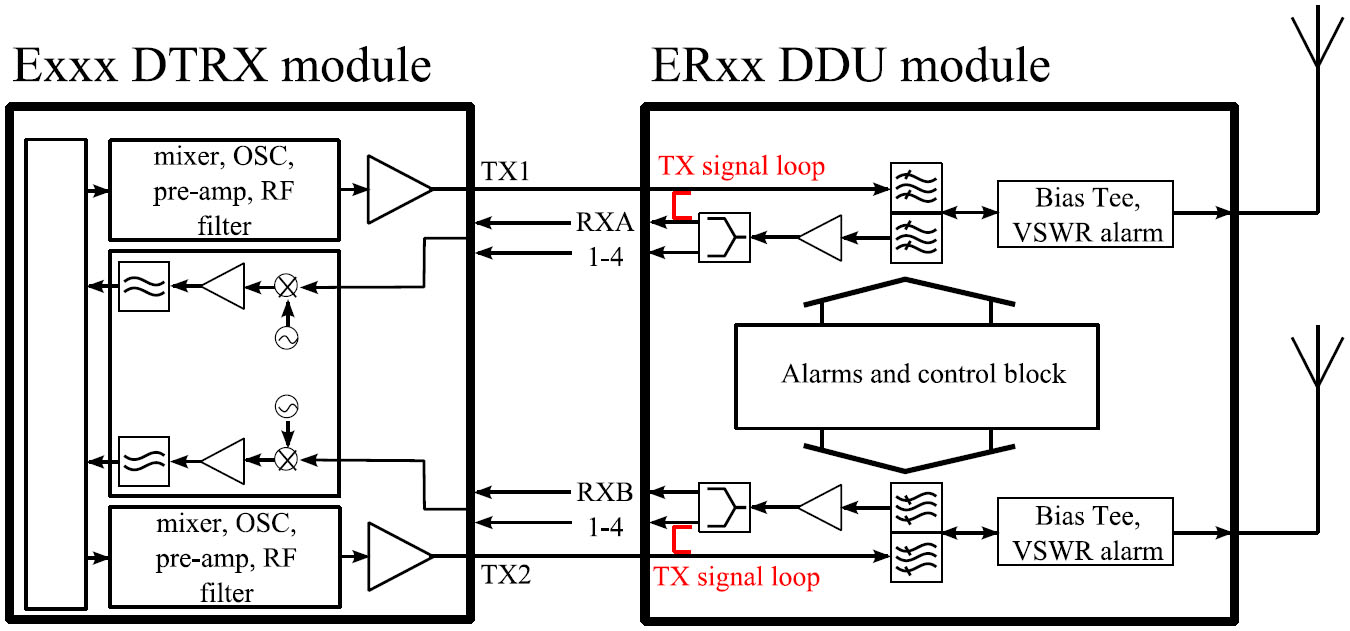
\includegraphics[scale=0.3]{img/bs.jpg}
	\caption{Receiver under study.}
	\label{f:bs}
	\end{center}
	\vspace*{-12pt}
\end{figure}

The laboratory consisted of four measrurement tasks. In the first task, the 1~dB compression 
point of the RX pre-amp block was measured at 900~MHz using both the spectrum analyzer and the 
VNA. The 1~dB compression point sets the limit to maximum power level of the received signal 
at input of the pre-amp block. In the second task, the gain of the RX pre-amp block was 
determined by measuring the 3~dB RX bandwidth of the block. The approximated equivalent 
noise bandwidth of the block and the TX-band attenuation were also measured. This task was 
already covered in the first lab assignment as a part of the diplexer characteristics. 

The third task is a noise measurement whose purpose was to determine the noise temperature of 
the RX pre-amplifier block using $Y$-coefficient method. Finally, the fourth task involving 
measuring the sensitivity of the RX pre-amplifier block, i.e., the minimum power level at 
input of the pre-amp block that can be detected with predefined $\textit{BER}$.

This report is divided in five sections. After this introduction, general measurement procedures 
are discussed. The third section presents the measurement results while the fourth section includes 
the error estimates. In the second to last section, some conclusions are drawn. Finally, feedback 
is also given in the last section to further improve this laboratory assignment of the course.


\newpage
\section{Measurement steps}

In this section, used measurement configurations are presented for each measurement 
task. Measurements in question may be divided into two distinct categories: power 
measurements with a spectrum analyzer (SA) and two-port transmission measurements ($S_{21}$)
with a vector network analyzer (VNA). There were no significant differences between 
the planned setups and those used in the actual measurements. The following 
measurement-specific subsections will elaborate.


\subsection{1~dB compression point}

To measure 1~dB compression point of a device, one needs a (manually) sweepable signal source 
and power detector. These may come separately or be incorporated in a single device. 
In both cases, the DDU module is connected the in between the source and the detector.
We used both approaches, and made two measurements with equal power levels.

For separate signal generation and detection, we used \textit{Rohde \& Schwarz SML03} signal 
generator (SG) and \textit{HP 8596E} spectrum analyzer.The measurement setup is shown in Figures 
\ref{f:sg1} and \ref{f:sg2}. The setup employing \textit{Rohde \& Schwarz ZVL} VNA is shown in 
Figures \ref{f:vna1} and \ref{f:vna2}. All equipment came precalibrated. In both measurements, 
the A-half of the base station was used.

\begin{figure}[h!]
	\begin{center}
	\setlength{\unitlength}{1mm}
	\begin{picture}(142, 13)
		\linethickness{0.2mm}
		\put(0, 0.4){\framebox[34mm]{Signal generator}}
		\put(34, 1.4){\vector(1,0){20}}
		\put(54, 0.4){\framebox[28mm]{$\mathrm{ANT} \rightarrow \mathrm{RX}_1$}}
		\put(82, 1.4){\vector(1,0){20}}
		\put(102, 0.4){\framebox[40mm]{Sprectrum analyzer}}
		\put(68, 7){\makebox(0,0){DDU module}}
	\end{picture}
	\vspace*{\halfLine}
	\caption{Measurement setup used in the first measurement task.}
	\label{f:sg1}
	\end{center}
	\vspace*{-12pt}
\end{figure}

\begin{figure}[h!]
	\begin{center}
	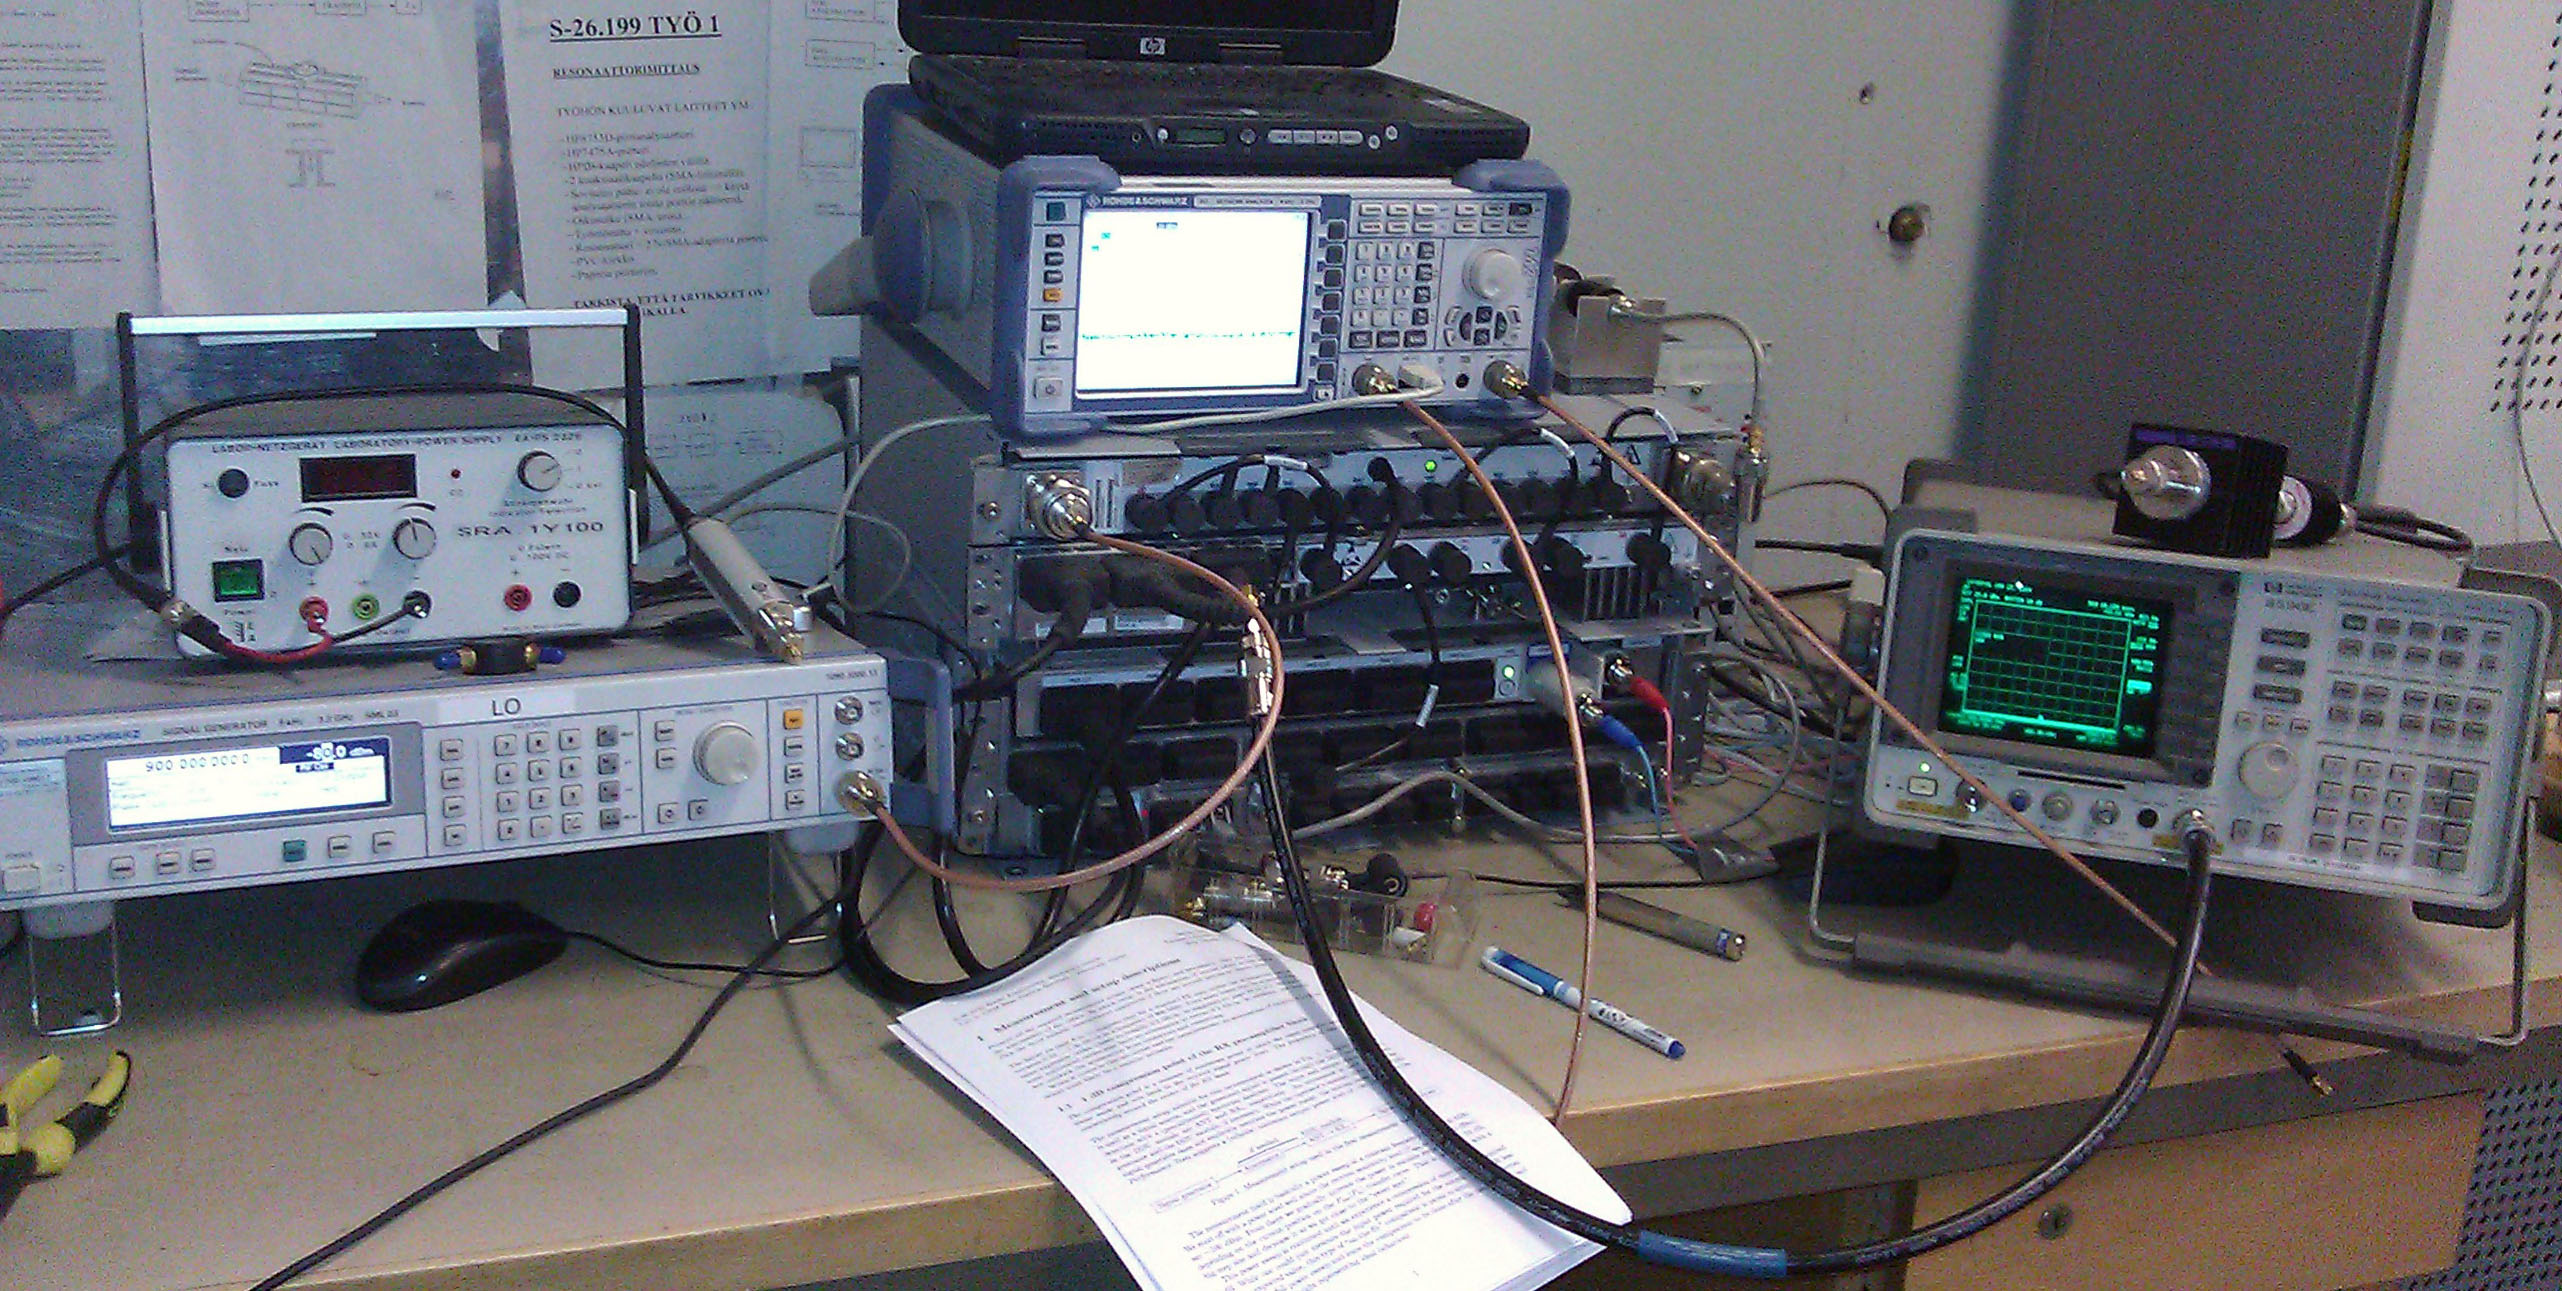
\includegraphics[width=0.75\textwidth]{img/sg-ddu-sa.jpg}
	\caption{Using a signal generator and spectrum analyzer to characterize the DDU module.}
	\label{f:sg2}
	\end{center}
	\vspace*{-12pt}
\end{figure}

\begin{figure}[h!]
	\begin{center}
	\setlength{\unitlength}{1mm}
	\begin{picture}(155, 10)
		\linethickness{0.2mm}
		\put(0, 0.4){\framebox[29mm]{VNA (Port 1)}}
		\put(29, 1.4){\vector(1,0){15}}
		\put(44, 0.4){\framebox[28mm]{$\mathrm{ANT} \rightarrow \mathrm{RX}_1$}}
		\put(72, 1.4){\vector(1,0){15}}
		\put(87, 0.4){\framebox[24mm]{Attenuator}}
		\put(111, 1.4){\vector(1,0){15}}
		\put(126, 0.4){\framebox[29mm]{VNA (Port 2)}}
		\put(58, 7){\makebox(0,0){DDU module}}
		\put(99, 7){\makebox(0,0){$L = 20$ dB}}
	\end{picture}
	\vspace*{\halfLine}
	\caption{VNA measurements connections}
	\label{f:vna1}
	\end{center}
	\vspace*{-12pt}
\end{figure}

\begin{figure}[h!]
	\begin{center}
	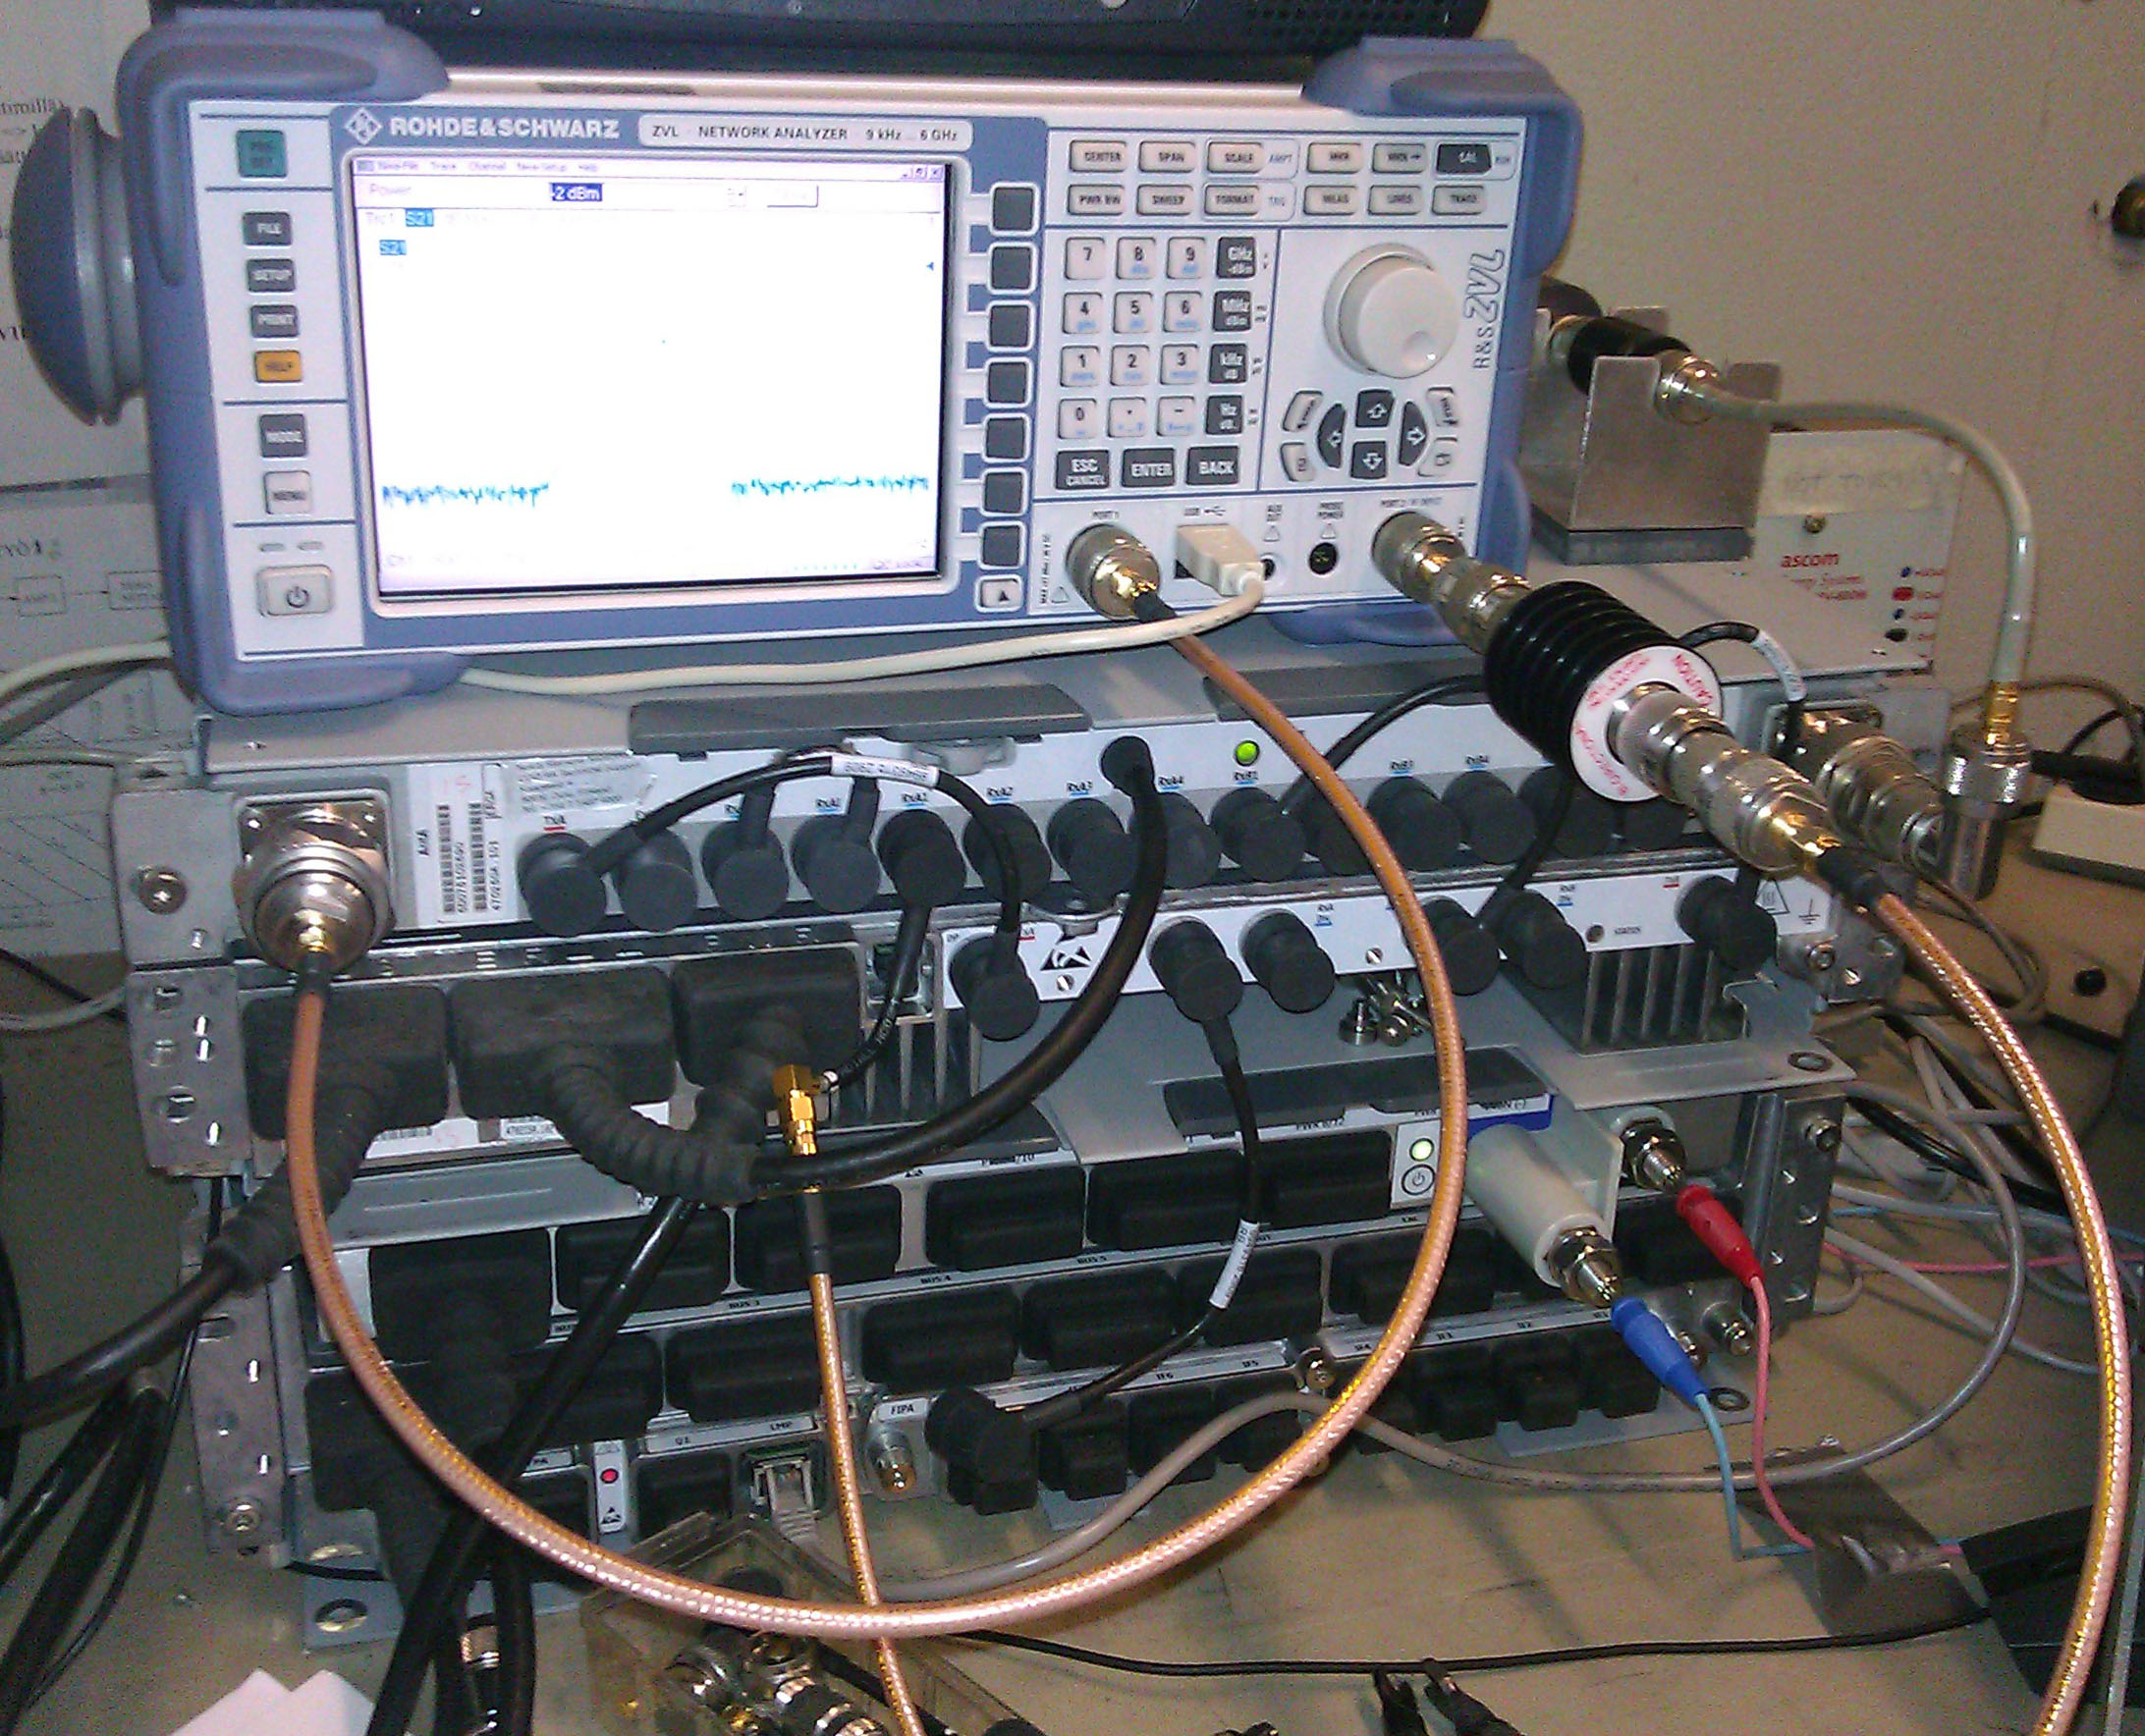
\includegraphics[width=0.75\textwidth]{img/vna-ddu-vna.jpg}
	\caption{Measuring the DDU module with the VNA.}
	\label{f:vna2}
	\end{center}
	\vspace*{-12pt}
\end{figure}

In essence, the measurement was a power sweep at a constant frequency of 
$f = 900$ MHz; mapping detected power or gain against used input power. 
This raw data was later postprocessed using Matlab.

We started with a source power of $-40$~dBm; a power level well below the 
1~dB compression point. The power was gradually used in steps of first 
10~dB, then 5~dB and finally 1~dB, until clear compression was observed. 
Compression may be seen in the lower than expected values of detected 
power (SG \& SA), or equivalently as lower gain (VNA).

Since we were measuring a GSM receiver, we used settings found in the GSM 
specification for the spectrum analyzer with the expeception of smaller 
averaging factor. The settings were as follows: an averaging factor of 100, 
zero span and 30~kHz video and resolution bandwidths. Input attenuation of the 
spectrum analyzer was increased from 10~dB all the way to 30~dB as we moved onto 
higher powers. 

The two cables and attenuators were measured separately using a VNA. For the VNA, 
the measurement settings throughout this lab were as follows: 1601 points over 
a frequency range of $800 \ldots 1000$~MHz, a measurement bandwidth of 10~kHz 
and averaging over 200 samples with a transmit power of $-20$~dBm.

For more accurate and/or reliable SA measurements, even a larger attenuation factor 
could have been used to avoid the small, yet possible, compression in the SA. One 
chould have also not trusted the quality of the SG as much than we did. The whole 
power sweep should have also been recorded without the DDU-module in between.
Also, there was some oversigth in making the connections as can be seen in 
Fig.~\ref{f:vna2}. As its only an attenuator in a transmission measurement, 
there is most likely no great an impact on the results as such. Nevertheless, 
it begs to question connector repeatability.


\subsection{Frequency response}

The frequency response was already measured in the first labs using a VNA. Thus 
we didn't need to measure the gain in these labs, as we used the results from 
the first labs. While the measurement procedure was given in the final report of 
the first labs, it is repeated here for completeness.

The measurement was carried out using a \textit{Rohde \& Schwarz ZVL} VNA, 
calibrated by the assistant prior to our arrival. The calibration settings were 
as follows: full two-port calibration with 1577 points within the $850 \ldots 1000$~MHz 
band, $-20$ dBm reference power, and an averaging factor of 100. The reference 
plane was located at the non-VNA end of the used cables.

The actual measurement included connecting the VNA to the B-half of the DDU module in 
order to obtain the values of $|S_{12}|$ over a set frequency range. In terms of physical 
connections, this would mean the following: VNA (Port~2) $\rightarrow$ DDU module 
(in: $\mathrm{ANT}_\mathrm{B}$, out: $\mathrm{RX}_\mathrm{B1}$) $\rightarrow$ VNA (Port~1). 
The raw data was stored onto a USB-memory as \texttt{*.s1p} files for post processing 
using Matlab.

The theoretical noise bandwidth $B_\mathrm{n}$ for a device may be found as using the 
following formula
\begin{equation}\label{e:Bn}
B_\mathrm{n} = \frac{1}{G_\mathrm{T,\;max}} \int_0^\infty G_\mathrm{T}(f) \, df,
\end{equation}
where $G_\mathrm{T}(f)$ is the transducer gain at frequency $f$. In practice, one may 
only approximate this using numerical integration over the finite measurement bandwidth. Such 
approximation is bound to yield slightly optimistic values. Another possibility is to 
approximate the noise bandwidth as the 3~dB bandwidth, and applying a compensation factor 
based on the transition bands. Results obtained using both methods are shown and compared 
later in the text.


\subsection{Noise temperature}

In the noise measurement task, we used the $Y$-coefficient method. The setup is shown 
in Figures \ref{f:nd1} and \ref{f:nd2}. A DC-voltage source is connected to a noise 
diode which is in turn connected by an SMA-cable to the $\mathrm{ANT}_\mathrm{A}$-input 
in the pre-amplifier block (A-half). It would have been better to use desired direct 
connection, but that was not possible due to missing adapters.

The signal is led then from the RX$_\mathrm{A1}$ output to the spectrum analyzer. We 
made another measurement where an amplifier was placed in between, as the noise power 
from the cold noise source might've been masked by the SA noise. The parameters of 
the amplifier, made by Minicircuits, were as follows: $B = 15 \ldots 3000$~MHz, 
$G = 19$~dB, $T = 463$~K, $F = 4.1$~dB and $V_\mathrm{CC} = +15$~V.

\begin{figure}[h!]
	\begin{center}
	\setlength{\unitlength}{1mm}
	\begin{picture}(163, 13)
		\linethickness{0.2mm}
		\put(0, 0.4){\framebox[10mm]{$V_\mathrm{DC}$}}
		\put(10, 1.4){\vector(1,0){12}}
		\put(22, 0){\framebox[25mm]{Noise diode}}
		\put(47, 1.4){\vector(1,0){12}}
		\put(59, 0.4){\framebox[28mm]{$\mathrm{ANT} \rightarrow \mathrm{RX}_1$}}
		\put(87, 1.4){\vector(1,0){12}}
		\put(99, 0.4){\framebox[12mm]{LNA}}
		\put(111, 1.4){\vector(1,0){12}}
		\put(123, 0.4){\framebox[40mm]{Sprectrum analyzer}}
		\put(5, 7){\makebox(0,0){0/28 V}}
		\put(73, 7){\makebox(0,0){DDU module}}
		\put(111, 8){\makebox(0,0){$\overbrace{\hspace{23mm}}^\textrm{with and without}$}}
	\end{picture}
	\vspace*{\halfLine}
	\caption{Noise temperature measurement setup}
	\label{f:nd1}
	\end{center}
	\vspace*{-12pt}
\end{figure}

\begin{figure}[h!]
	\begin{center}
	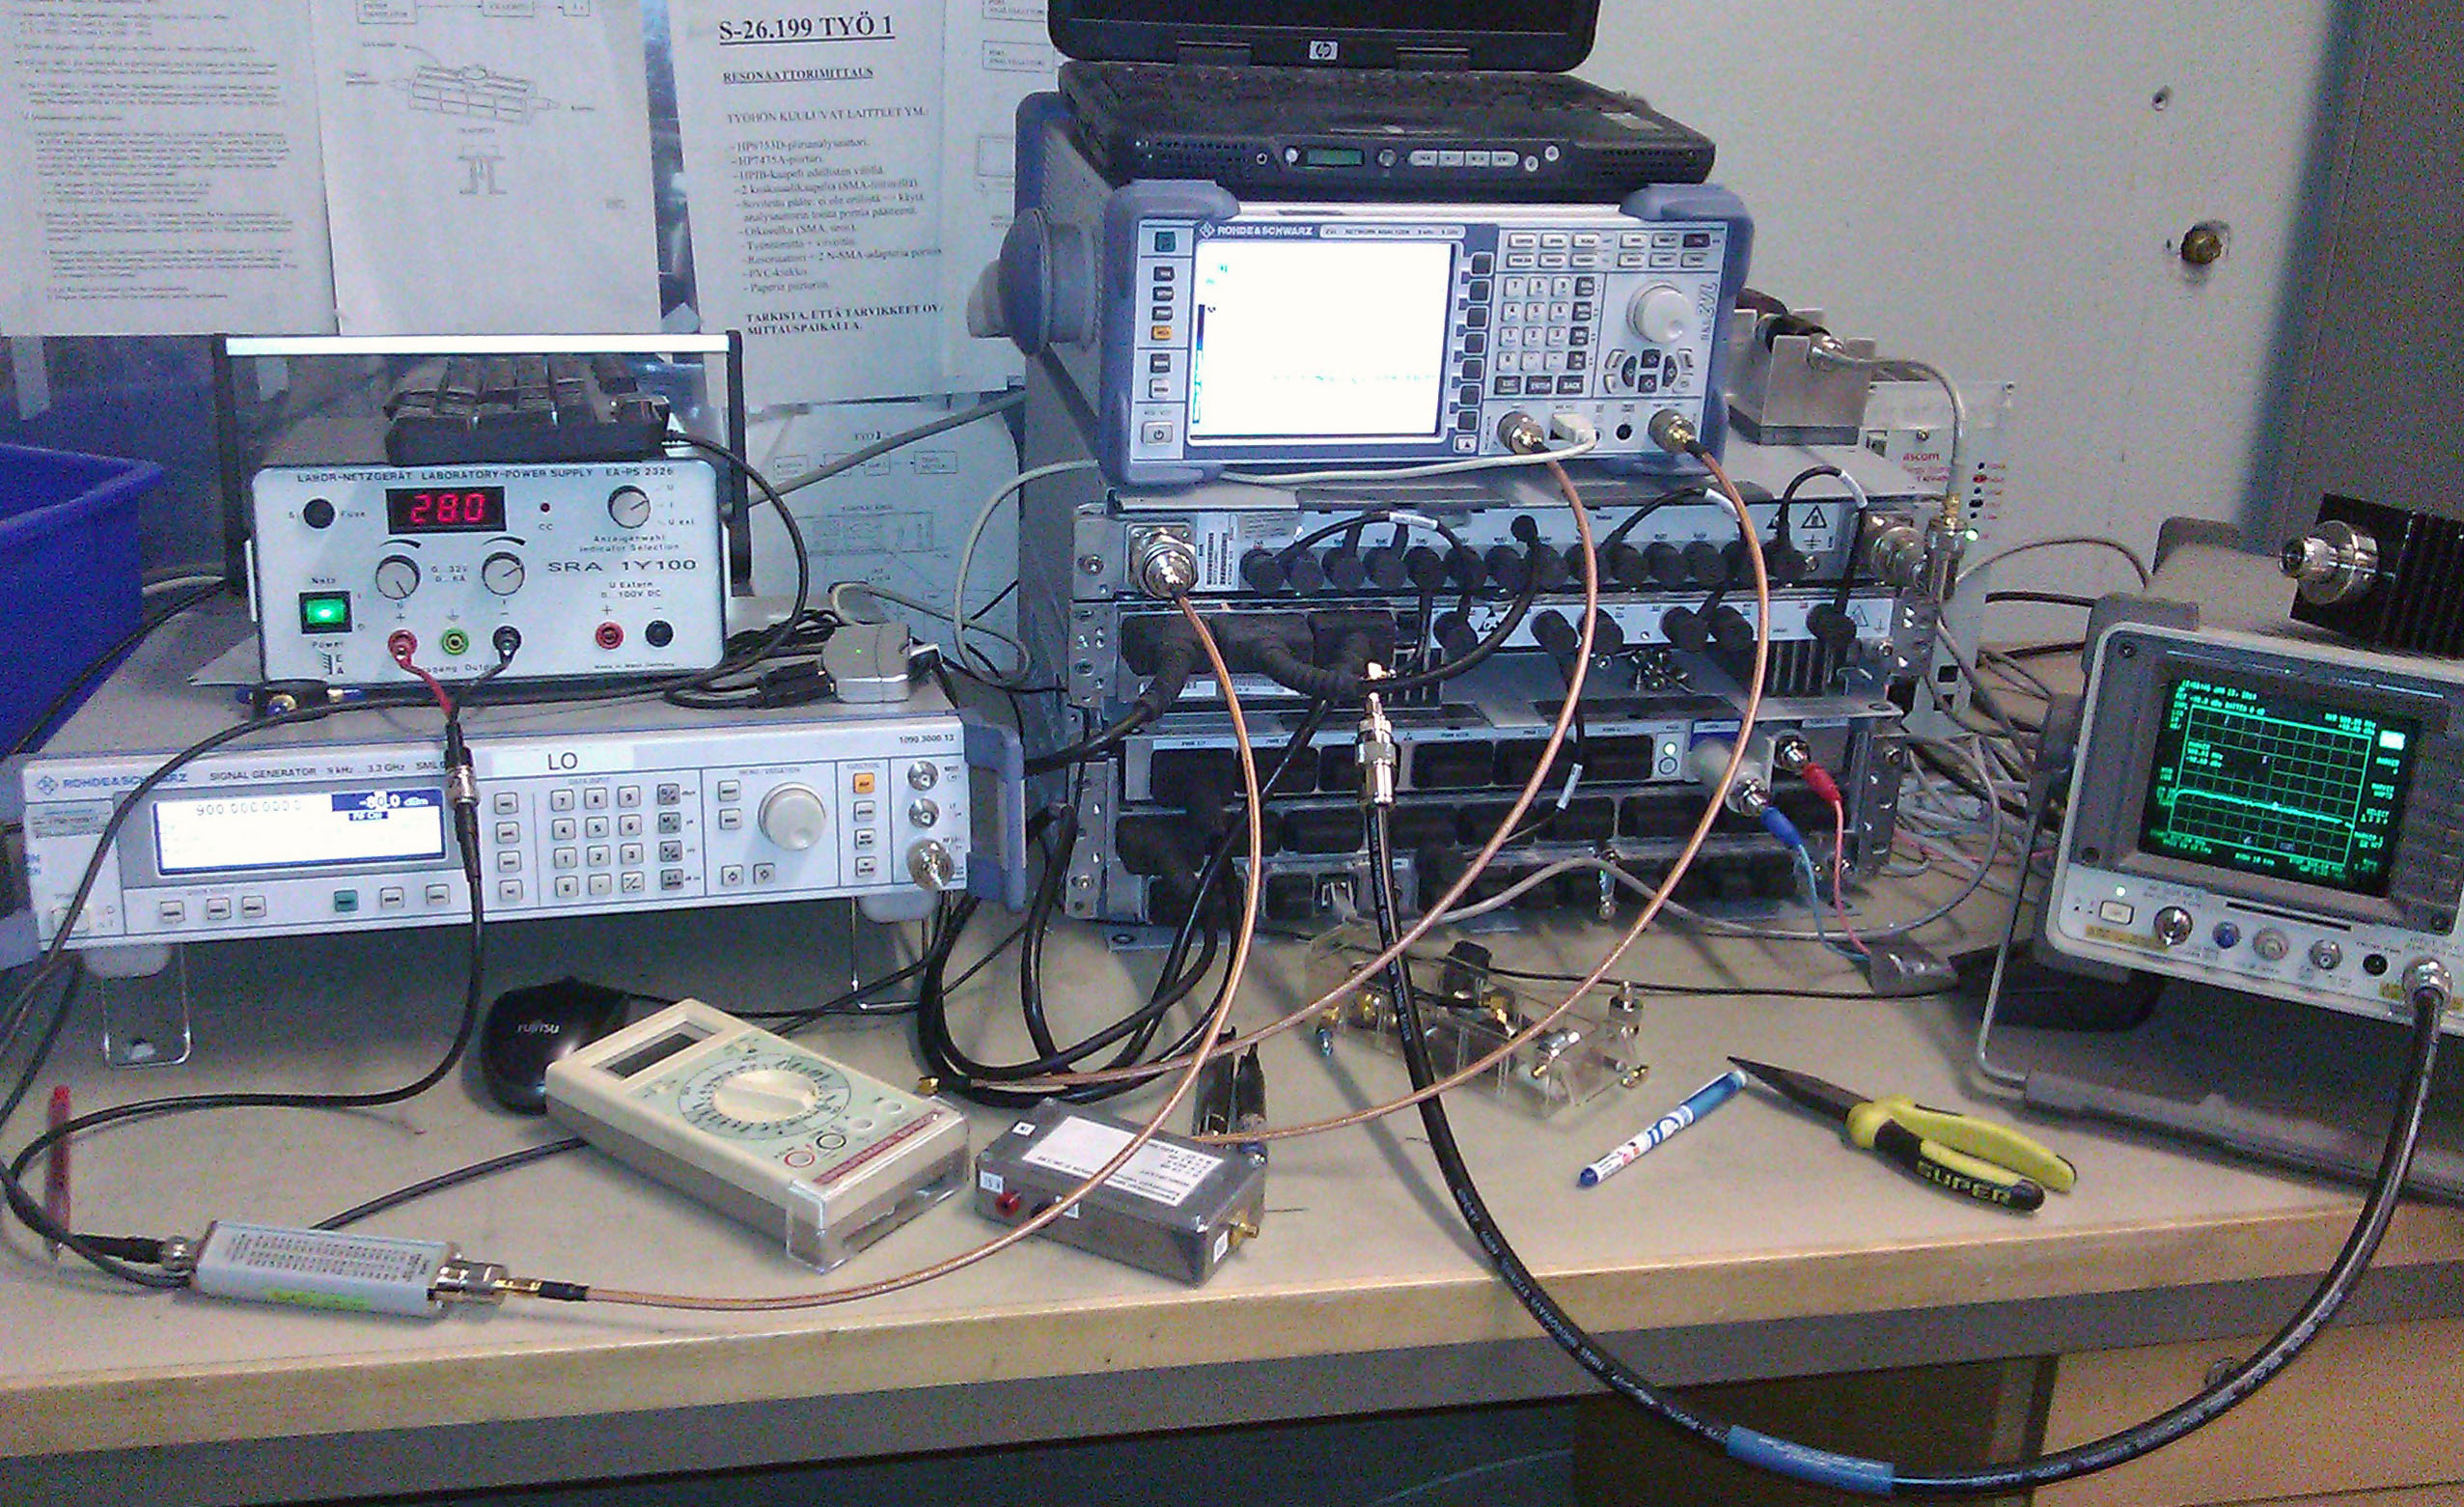
\includegraphics[width=0.75\textwidth]{img/nd-ddu-sa.jpg}
	\caption{Noise temperature measurement setup without the additional amplifier.}
	\label{f:nd2}
	\end{center}
	\vspace*{-12pt}
\end{figure}

The measurements themselves were carried out measuring two power levels required in the 
Y-pa\-ram\-e\-ter; when the DC-voltage is off/shorted (``cold'') and on (``hot''). We 
used \textit{HP 346B} noise diode ($\textit{ENR} = 21.48$~dB when $f = 1.00$~GHz) with 
a control voltage of 28~V$_\mathrm{DC}$ taken from a laboratory-grade voltage source.

As for the SA settings, the settings we as follows: 0~dB input attenuation, zero span, 
10~kHz resolution and video bandwidths and an averaging over 100 sweeps. For more accurate 
results, more time should have spent on this measurement. This would have allowed us to use 
smaller bandwidths and larger averaging factor.

The noise temperature, or equivalently noise factor/figure, may be found using the following
formulae. $Y$-coefficient is given as
\begin{equation}\label{e:Y}
Y = \frac{P_\mathrm{H}}{P_\mathrm{C}} 
	= \frac{T_\mathrm{H} + T_\mathrm{e}}{T_\mathrm{C} + T_\mathrm{e}}
	\quad\Rightarrow\quad
	T_\mathrm{e} = \frac{T_\mathrm{H} + YT_\mathrm{C}}{Y - 1},
\end{equation}
where $P_\mathrm{H/C}$ is the measured power for hot and cold loads at equivalent noise 
temperatures $T_\mathrm{H/C}$, and $T_\mathrm{e}$ is the noise temperature of the measured 
device. $T_\mathrm{C} = 290$~K is the physical temperature of the noise diode, and 
$T_\mathrm{H}$ may be solved from the definition of $\textit{ENR}$:
\begin{equation}\label{e:ENR}
\mathit{ENR} = 10 \lg \left( \frac{T_\mathrm{H}}{T_\mathrm{0}} - 1 \right) 
	\quad\Rightarrow\quad
	T_\mathrm{H} = T_\mathrm{0} \left( 10^\frac{\mathit{ENR}}{10} + 1 \right).
\end{equation}
Obtained noise temperature $T_\mathrm{e}$ may be converted to noise factor $F$ or figure 
$F_\mathrm{dB}$ using the following relationship:
\begin{equation}
F_\mathrm{dB} = 10 \lg \left( F \right) \mathrm{\;dB} =  10 \lg \left( 1 + \frac{T_\mathrm{e}}{T_0} \right) \mathrm{\;dB}.
\end{equation}

One should notice that the $T_\mathrm{e}$ given by Eq.~\ref{e:Y} is actually the noise 
temperature of the whole chain. This chain is a cascaded system, consisting of a SMA-cable, 
the DDU module, the optional amplifier, another SMA-cable and the spectrum analyzer, in 
this order. The contribution of the DDU module may be determined by reverse calculating 
Friis' noise equation:
\begin{equation}\label{e:Friis}
	F_\mathrm{total} = F_1 + \frac{F_2 - 1}{G_1} + \frac{F_3 - 1}{G_1 G_2} + \cdots
	\quad\Leftrightarrow\quad
	T_\mathrm{total} = T_1 + \frac{T_2}{G_1} + \frac{T_3}{G_1 G_2} + \cdots,
\end{equation}
where $G_i$ is the available power gain of the $i$th stage. Similar indexing is also used 
for both of the noise quantities $F$ and $T$. This simplified formula assumes equal noise 
bandwidths between the stages.

The parameters required by the formula may be obtained through calculation, or are provided 
by the manufacturer. For example the noise contribution of the cables can be obtained from 
their attenuation $L$ and physical temperature $T_\mathrm{phys}$ through formula 
$F = (L - 1) T_\mathrm{phys}$. The amplifier specifications were given already in the text.
For the spectrum analyzer, its noise noise characteristics eluded us. Luckily, there is 
significant gain earlier in the chain, thus minimizing the effect of the noise originating 
in the SA.


\subsection{Sensitivity}

In the sensitivity measurement, we measured the minimum input power at the ANT$_\mathrm{A}$-input 
that results in a reliably detectable signal above the noise floor in the ouput of the DDU module. 
In GSM-systems, a signal with $\mathit{SNR} > 10$~dB is detected with an acceptable $\mathit{BER}$. 
For this, a measurement setup identical to the one used in the first task may be used. The setup 
used there is shown in Figures \ref{f:sg1} and \ref{f:sg2}. An attenuator may be used between 
the signal generator and the DDU module.

\begin{figure}[h!]
	\begin{center}
	\setlength{\unitlength}{1mm}
	\begin{picture}(142, 13)
		\linethickness{0.2mm}
		\put(0, 0.4){\framebox[34mm]{Signal generator}}
		\put(34, 1.4){\vector(1,0){20}}
		\put(54, 0.4){\framebox[28mm]{$\mathrm{ANT} \rightarrow \mathrm{RX}_1$}}
		\put(82, 1.4){\vector(1,0){20}}
		\put(102, 0.4){\framebox[40mm]{Sprectrum analyzer}}
		\put(68, 7){\makebox(0,0){DDU module}}
	\end{picture}
	\vspace*{\halfLine}
	\caption{Measurement setup used in the sensitivity measurement.}
	\label{f:m4}
	\end{center}
	\vspace*{-12pt}
\end{figure}

The first step was to measure the noise floor at 900~MHz without any signal 
we're hoping to detect. That is, the RF power was switched off at the generator. 
Then we turned on an input signal that's some dBs below the reported sensitivity 
level of $-112.5$~dBm. We gradually increased the power until the signal-to-noise 
ratio was no less than the 10~dB required by the standard. The corresponding power 
level was recorded. Also powers corresponding to an $\textit{SNR}$ of 12.5 and 7.5~dB 
we measured. 

One could have also measure the power required to beat the noise just barely, and 
add the SNR later on. This approach is, however, less accurate and more painful. It 
also assumes $P_\mathrm{out}(P_\mathrm{in})$ relationship to be ideal in the range.

Since it's a GSM system, we use the measurement settings as they are defined in 
the standard with the exception of averaging. The standard 500-sweep averaging was 
used in when measuring the noise floow, but 100 was used when RF power was enabled. 
The final settings were as follows: an averaging factor of 500/100, zero span and 
30~kHz video and resolution bandwidths. The input attenuator was disabled in the 
SA settings.


\newpage
\section{Results}

The results are described in detail in the following subsections. The four measurement 
data were post-processed either by Matlab or by means of calculation to find wanted 
parameters of the pre-amp block under test.

The attenuation of cables and attenuator used in the measurements were determined using 
the VNA, and were taken into account when post-processing the measurement data. The 
attenuations are $19.95$~dB, $0.2$~dB and $0.3$~dB, for the attenuator, thin cable and 
thick cable, respectively. The parameters of the additional amplifier used in the noise 
measurement were specified as follows: $G = 19$~dB, $T = 463$~K, $F = 4.1$~dB.


\subsection{1~dB compression point}

1~dB compression point arises from the nonlinearities of the receiver LNA. At high enough 
powers, the gain of the LNA for a certain frequency starts to drop with increasing power. 
The input power at which the LNA gain is compressed by 1~dB was measured using two different 
measurement setups. The results are presented here.

The first measurement setup consisted of a signal generator and a spectrum analyser. A single 
frequency of 900~MHz sent from the signal generator was measured with the spectrum analyser. 
The signal generator power was increased gradually, until a 1~dB drop in the gain was achieved. 
The measurement results for the first setup are presented in Fig.~\ref{f:1dB}(a, c and e). 
The attenuations of the cables are corrected from the results.

The second measurement setup consisted of a vector network analyser. The VNA was measuring 
the $|S_{21}|$ as the input power was increased gradually, until a 1 dB~drop was visible 
on the screen. An attenuator was required in between the base station and VNA port 2 
to protect the device from the amplified signal. The measurement results for the second setup 
are presented in Fig.~\ref{f:1dB}(b, d and f). The vector network analyser was calibrated 
before use. 

All the sub figures are plotted from one data set for spectrum analyser setup and VNA setup each. 
The data sets are post processed using Matlab. Both data sets are visualised with three different 
figures, so that it is easier to compare the two measurements. Matlab \textit{'phcip'} interpolation with 
additional extrapolation was used for completeness. The Extrapolated data should not thus be taken 
into account when analysing the DDU performance.

The compression point derived from the spectrum analyser measurement is \linebreak{}$CP_\mathrm{a} = -5.6$~dBm. 
Fig. \ref{f:1dB}(c) shows how the measured gain fluctuates around the average gain of 24.6~dB, 
however, with a small amplitude. The compression point derived from the VNA measurement is 
$CP_\mathrm{b} = -4.1$~dBm without any gain fluctuation. One could assume the ``actual'' 
compression point to be found within these limits.


\begin{figure}
\centering
\subcaptionbox{$P_\mathrm{out}(P_\mathrm{in})$ using SG \& SA}{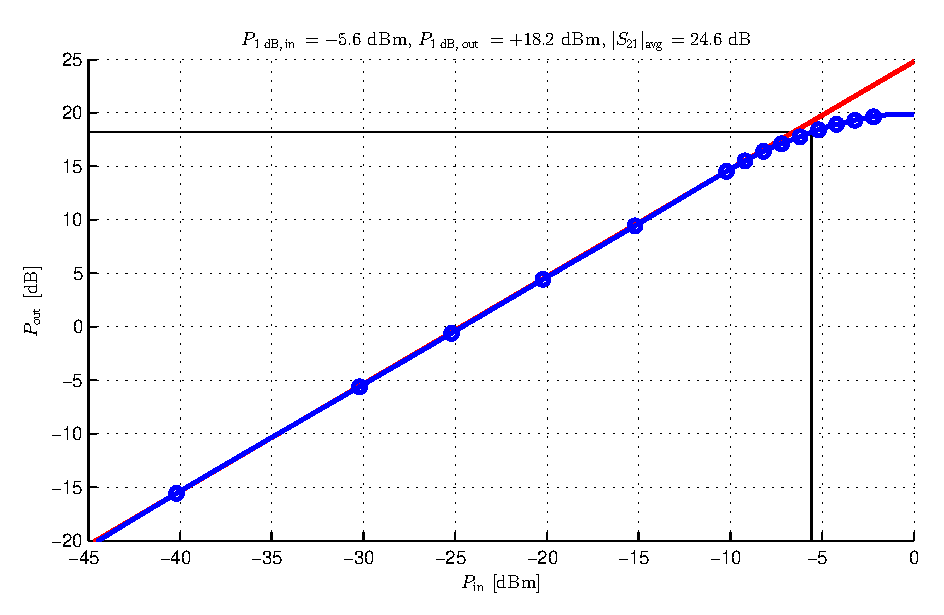
\epsfig{file=img/PoutPin1.eps, width=0.45\textwidth}}
\subcaptionbox{$P_\mathrm{out}(P_\mathrm{in})$ using VNA}{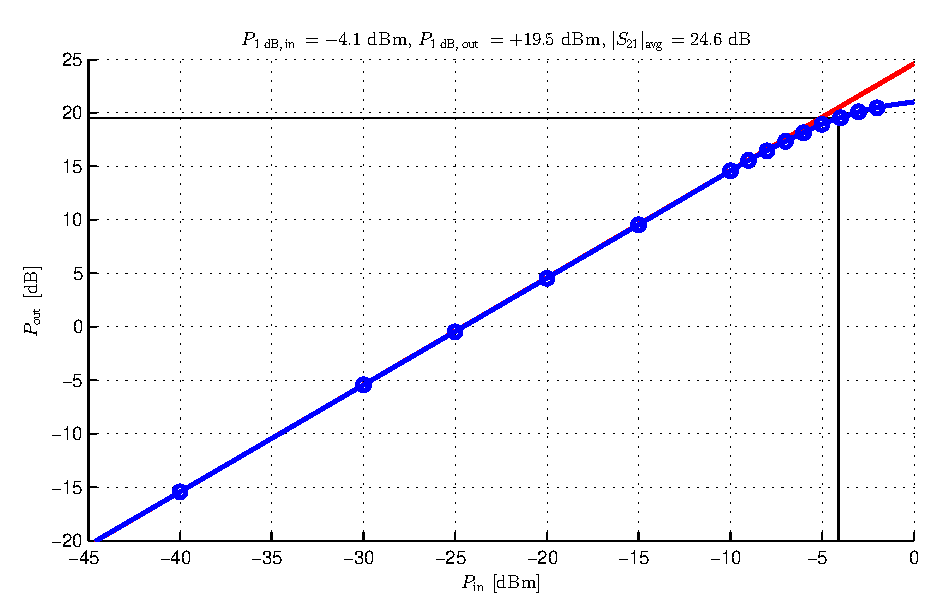
\epsfig{file=img/PoutPin2.eps, width=0.45\textwidth}}
\subcaptionbox{$G(P_\mathrm{in})$ using SG \& SA}{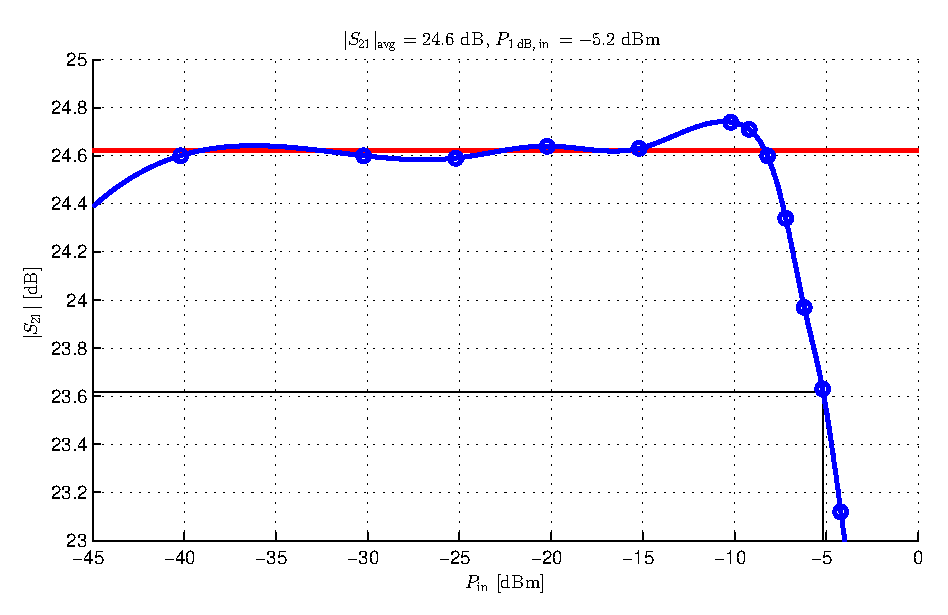
\epsfig{file=img/GPin1.eps, width=0.45\textwidth}}
\subcaptionbox{$G(P_\mathrm{in})$ using VNA}{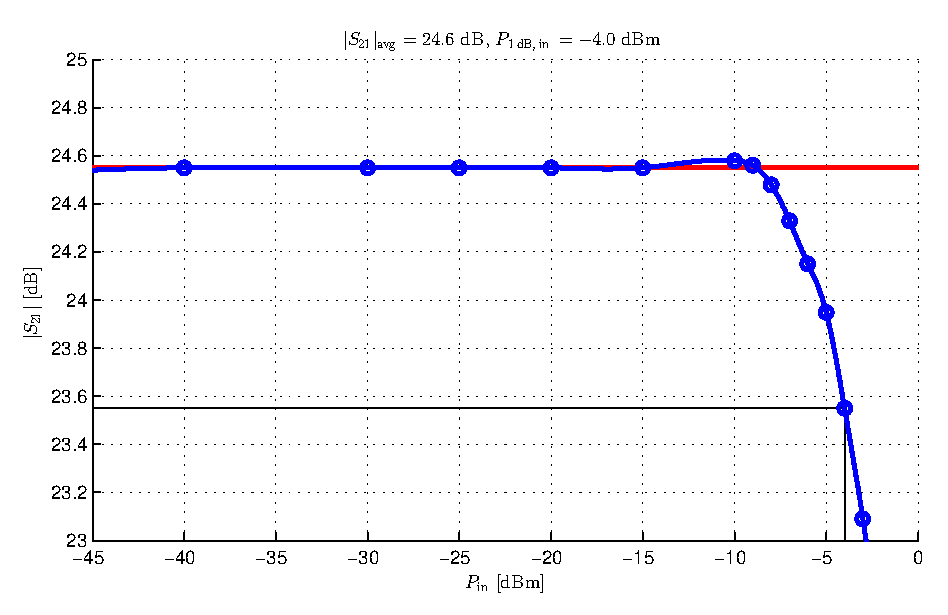
\epsfig{file=img/GPin2.eps, width=0.45\textwidth}}
\subcaptionbox{$G(P_\mathrm{out})$ using SG \& SA}{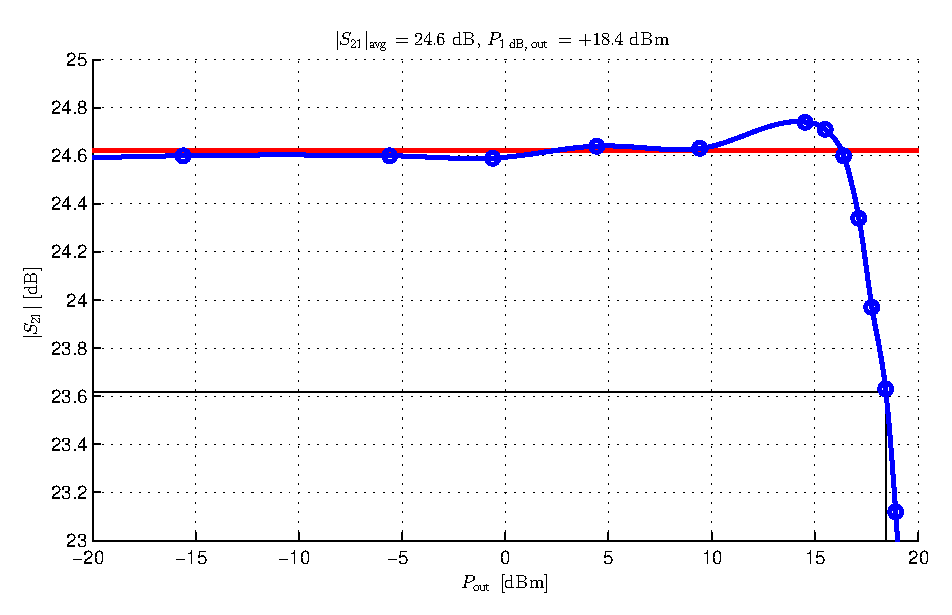
\epsfig{file=img/GPout1.eps, width=0.45\textwidth}}
\subcaptionbox{$G(P_\mathrm{out})$ using VNA}{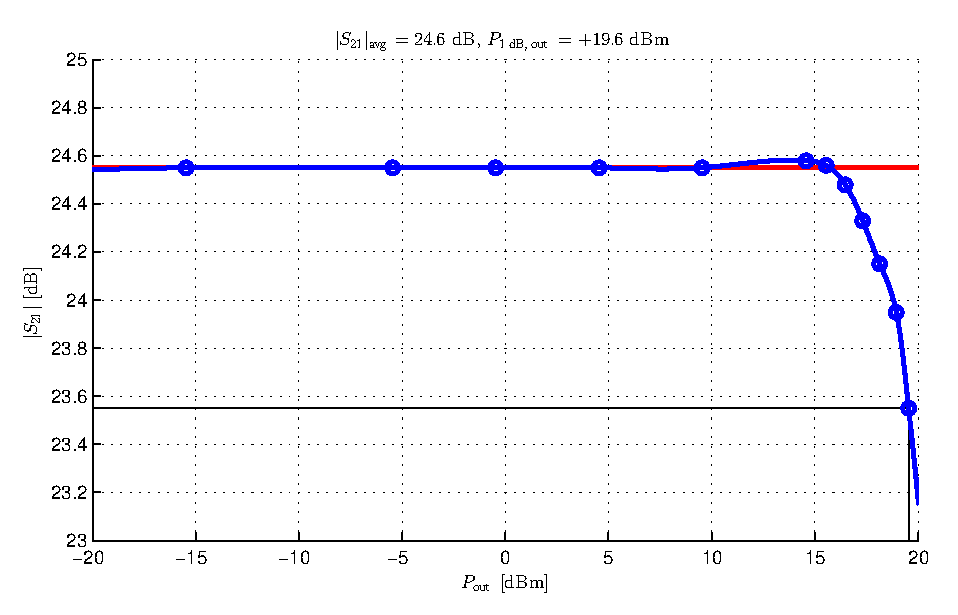
\epsfig{file=img/GPout2.eps, width=0.45\textwidth}}
\caption{Results from the 1~dB compression point measurements. Ideal behaviour is shown with red straights, 
	measuremets with blue markers and Matlab \texttt{'pchip'} interpolant in blue.}\label{f:1dB}
\end{figure}

\newpage
\subsection{Frequency response}

The $|S_{12}|$ response of the DDU module (B-half) within the $850 \ldots 1000$~MHz band 
is shown in the following figure (Fig.~\ref{f:s12}). In the figure, in addition to the 
actual response (in black), additional information is shown. GSM RX and TX band limits 
(in red), both 3~dB (in blue) and noise (in green) bandwidth of the pre-amp block are also 
visualized. Visualization of the noise bandwidth is somewhat questionable as it's a purely 
theoretical concept, but is nevertheless shown for scale. 

\begin{figure}[h!]
	\begin{center}
	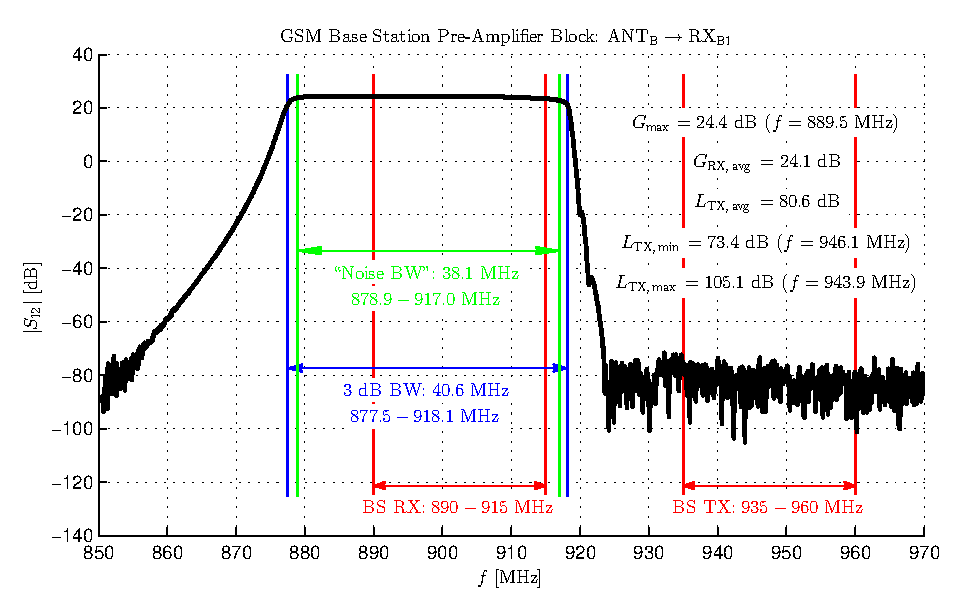
\epsfig{file=img/s12.eps, width=\textwidth}
	\caption{$S_{12}$ of the DDU module as was measured in the first labs.}
	\label{f:s12}
	\end{center}
	\vspace*{-12pt}
\end{figure}

The noise bandwidth shown, obtained from Eq.~\ref{e:Bn} is less than the actual band since 
we cannot use infinite frequency range. Frequency range of $850 \ldots 1000$~MHz with
$G_\mathrm{T,\;max} = |S_{12}|_\mathrm{max} = 24.4$~dB was used instead. The obtained 
value (38.1~MHz) is roughly 6~\% shy of the 3~dB bandwidth (40.6~MHz), as one might expect.
The 3~dB bandwidth may thus be used to avoid being overly optimistic.

In the graphical approximation method we need to investigate the effect of frequency 
roll-off speed. From Fig.~\ref{f:s12} the transition bands are approx. 30~MHz (3.4 \%) 
and 5~MHz (0.55 \%) for lower and upper bands, respectively. During this transition, 
the $S_{12}$ drops roughly 100~dB from $+20$~dB to $-80$~dB. This corresponds to a slope 
of $3.3$~dB/MHz (29~dB/\%) and $-20$~dB/MHz ($-180$~dB/\%), respectively. The effect of 
such steep slopes are neglectable, and thus the 3~dB bandwidth may be used as the noise 
bandwidth.


\subsection{Noise Temperature}

\noindent
The noise of the RX block was measured two times using the Y coefficient method, the noise diode
working as a hot load and a short circuit as a cold load in room temperature (290~K). The first 
measurement was done without an extra LNA in between the spectrum analyser and the RX block, and 
the second measurement was done with the LNA in between.

The noise temperature of the hot load can be calculated from the $\mathit{ENR}$ using Eq. \ref{e:ENR}, which 
gives $T_\mathrm{H} = 41065$~K. The equivalent noise temperature of the chain in between the diode and 
the spectrum analyser can be calculated from this temperature, room temperature and the measured 
noise powers. This is done using the $Y$-coefficient method, which gives $T_{\mathrm{total,\;w/}} = 162.1$~K 
and $T_{\mathrm{total,\;w/o}} = 643.8$~K for the setups with and without the LNA, respectively.

The previous noise temperature values still include the noise powers from the other parts of the 
chain, i.e., cables, the LNA and the SA. The RX block noise temperature can be obtained from Eq.~\ref{e:Friis},
which is for example for the LNA setup

\begin{equation}
T_\mathrm{total,\;w/} = T_\mathrm{C1} + L_\mathrm{C1} T_\mathrm{DDU,\;w/} + \frac{L_\mathrm{C1} T_\mathrm{LNA}}{G_\mathrm{DDU}} + \frac{L_\mathrm{C1} T_\mathrm{C2}}{G_\mathrm{DDU} G_\mathrm{LNA}},
\end{equation}

\noindent
and yields $T_{\mathrm{DDU,\;w/}} = 139.7$~K and $T_{\mathrm{DDU,\;w/o}} = 601.4$~K for the setups 
with and without the LNA, respectively. Subscript $\mathrm{C}i$ refers to the $i$th cable.

\begin{table}[!h]
	\begin{center}
	\caption{Results from the noise measurement.}
	\label{t:noise}
	\renewcommand*{\arraystretch}{1.2}
	\begin{tabular}{cccccc}
	LNA? 			& $P_\mathrm{C}$ [dBm] 		& $P_\mathrm{H}$ [dBm]	& $T_\mathrm{total}$ [K] 	& $T_\mathrm{DDU}$ [K] 	& $F_\mathrm{DDU}$ [dB] \\
	\hline
	No				& $-107.3$					& $-90.8$				& $643.8$ 							& $601.4$ 						& $4.9$\\
	Yes				& $-91.3$					& $-71.7$				& $162.1$ 							& $139.7$ 						& $1.7$ 	
	\end{tabular}
	\end{center}
	\vspace*{-12pt}
\end{table}


The final results are presented in Table \ref{t:noise}. The results differ significantly. The noise 
temperature calculated from the LNA setup is clearly closer to reality than the result obtained without 
the LNA. The reason for this is that the cold noise power is does not exceed the noise floor of the SA 
with a large enough margin. The LNA is required in the setup to rise the noise level high enough, so 
that it can be defined more precisely with the spectrum analyser.


\subsection{Sensitivity}

In this measurement, the sensitivity or the minimum detectable input power of the RX pre-amp block 
was measured using SA. The noise level at the output of the block was measured, when the RF power from 
SG was completely turned off, to be at $-101.89$~dBm. Three different output SNR values of the block, 
the minimum \textit{SNR} from GSM standard, below GSM minimum standard and above GSM minimum standard, 
were used to calculate desired power level at the output side. Input power levels from SG were written 
down when the desired output powers were reached. Table \ref{t:sens} below summarizes the 
measurement data for the minimum detectable input power at different values of $\textit{SNR}$.

\begin{table}[!h]
	\begin{center}
	\caption{Results from the sensitivity measurement.}
	\label{t:sens}
	\renewcommand*{\arraystretch}{1.2}
	\begin{tabular}{cc}
	$\mathit{SNR}$ [dB] 			& $P_\mathrm{transmit}$ [dBm]  \\
	\hline
	7.5								& $-118.0$ 	\\
	10								& $-115.6$ 	\\
	12.5							& $-113.0$ 	
	\end{tabular}
	\end{center}
	\vspace*{-12pt}
\end{table}

It can be seen that at the minimum SNR required from GSM standard (around 10 dB) the measured 
sensitivity of the RX pre-amp block is $-115.6$~dBm. Taking into account the attenuations caused 
by SMA-cables, which were measured in the first task, the actual sensitivity is $-116.1$~dBm 
(${\!\!}=-115.6\mathrm{\;dBm} - 0.2\mathrm{\;dBm} - 0.3\mathrm{\;dBm}$). 

These results assume the SA recognizes its measuring noise and applies internal correction. Most 
likely this correction must be done manually by adding 2.5~dB to the noise floor. \cite{kakkaa_huuleen} 
The same effect may achieved by using an SNR of 12.5~dB, resulting in a sensitivity level of $-113.6$~dBm.

\subsection{Dynamic range}

The dynamic range of a radio receiver is a range of received signal levels over which the receiver 
can operate. The dynamic range of the DDU under test can be determined as a ratio of the 1~dB 
compression point and the sensitivity or the minimum detectable power (MDP) of the pre-amp block. 
In decibels, the dynamic range is simply a difference between these two power limits:
\begin{equation}
\mathit{DR} = P_\mathrm{1\;dB} - P_\mathrm{MDP} 
\end{equation}
Using the values of the 1~dB compression point and the sensitivity obtained from measurement, the 
measured dynamic range of the RX pre-amp block is:
\begin{equation}
\mathit{DR}_\mathrm{measured} = -5.6 \mathrm{\;dBm} - (-116.1 \mathrm{\;dBm}) = 110.5 \mathrm{\;dB}
\end{equation}
The theoretical value of dynamic range is calculated with the provided sensitivity from producer as 
following:
\begin{equation}
\mathit{DR}_\mathrm{theoretical} = -5.6 \mathrm{\;dBm} - (-112.5 \mathrm{\;dBm}) = 106.9 \mathrm{\;dB}
\end{equation}

The measured 1~dB compression point value was applied in the theoretical dynamic range calculation 
above, since there is no such value given by producer. Therefore, the theoretical and measured dynamic 
ranges differ by $-3.6$~dB due to different sensitivity values as discussed in the 
previous subsection.

These measurements we obtained using the 1~dB compression point from the SG \& SA measurement along 
with the assumption that the spectrum analyzer makes the noise correction. Using 1~dB compression point 
obtained from the VNA measuremens indcreases both dynamic ranges by 1.5~dB. Correcting for the noise 
decreases $\mathit{DR}_\mathrm{measured}$ by 2.5~dB.


\newpage
\section{Error estimates}

In this section, error estimates for the two types of measurements are presented.
The values presented here are only rough estimates based on literature (with more 
or less general cases) and their soundness in this case is somewhat questionable. 
In this section, we do not take human errors (see previous section) into account. 
It is just stated that systematic errors arising from the cables and connections 
are possible in measurement all measurements. Thus they are valid only for 
``correct'' measurements, and are more of the ``provided for completeness'' 
nature. Propabilities are not given due to the nature/basis of the estimation.


\subsection{Spectrum analyzer}

Each of the components inside the spectrum analyzer contributes to the total uncertainty, 
depending for example on the signal frequencies, amplitudes, and measurement settings. 
The Agilent (former HP, manufacturer of the used SA) has made available a document that 
specifies the different error sources, giving also rough estimates for some spectrum 
analyzers. According to the document \cite{sa}, the error estimates vary broadly among 
different analyzer models, giving worst case uncertainties exceeding $\pm 6$~dB. On the 
other hand, the document gives also representative values of amplitude uncertainties, 
which in our case yields about $\pm 1$ dB.

The second error source for the spectrum analyzer is the power marker reading. In 
each of the tasks, the spectrum analyzer was set to average 500 measurement points, 
which should average out most of the random errors. However, reading the power marker 
in the screen, there was a noticeable fluctuation in the shown power value. Based on the 
experience obtained during the measurements, the power marker error is estimated to be 
approximately $\pm 0.5$ dB.

In conclusion, the error estimates that can be taken into account numerically are 
the manufacturers representative value of approx. $\pm 1$ dB, and the power marker 
fluctuation of roughly $\pm 0.5$ dB. These uncorrelated errors may be summed to 
achieve the total uncertainty of the SA measurements of approx. $\pm 1.5$ dB. 

There is also the question of calibrating the spectrum analyzer properly with 
the time interval defined by the manufacturer. Agilent suggests to have the spectrum 
analyzer calibrated thoroughly once in a year, and quick-calibrated if there are 
changes operating environment \cite{sa2}. If the spectrum analyzer used in the 
measurements is not calibrated correctly, it is possible that the measurements are 
not reliable. In this case, the calibration is the most important error source, and 
the device should be calibrated correctly before estimating any other errors.


\subsection{Vector network analyzer}

For the VNA, different error sources and ways to cope with them are listed in the 
lecture slides discussing VNA measurements. The different sources are noise, 
cabling/connector repeatability, directivity, isolation, mismatch and environment 
induced drift. 

Noise and cabling/connector repeatability are random errors, which can be averaged 
out. In our case, only the noise was averaged, since we did not touch the cabling. 
Systematic errors arising directivity, isolation, and mismatch in this task were
for the most part neglected with a calibration. Before conducting measurements, 
the VNA is always calibrated using a standard calibration module. The calibration 
moves the reference planes to the connectors of the test cables, and somewhat 
cancels the systematic errors from the connectors and cables used in a specific 
measurement. Finally, the environment induced drift is not relevant, since the 
measurement was done inside a short time interval.

Rohde \& Schwarz provides specifications that describe the measurement uncertainty 
of the VNA in question in different frequency bands. For transmission measurements 
in the frequency range of 50 MHz to 3 GHz, accuracy for signal powers of $-50 \ldots 0$ 
dB is better than $0.2$ dB ($0.3$ dB for powers of $-50 \ldots {-70}$ dB) with 0~dBm 
transmit power. \cite{vna} The reader should note that these ranges was exceeded 
from both ends during the measurements (the measurement power range was roughly 
$-100 \ldots {+4}$ dBm). 

In conclusion, two things are assumed. First, calibration is assumed to cancel the 
systematic errors arising from cables and connectors to a neligible level. Second, 
random errors are cancelled with averaging almost entirely. The manufacturer provides 
error estimates for the device itself, giving an error estimate of under $0.3$ dB that 
is mostly applicable in our case. The topics discussed in the last paragraph of the 
last subsection apply here to some extent to here as well.


\subsection{Noise diode}

According to the lecture supplement handout \cite{kakkaa_huuleen}, error sources in noise 
measurements can be divided into four categories. First error source is the noise diode 
calibration error, second error source arises from $Y$-factor method, third from mismatches 
and fourth from the attenuations. Also the physical operating temperatures might have been 
some kelvins above $T_0 = 290$~K.

The noise diode calibration uncertainty is about $\pm0.1$~dB. The noise diode ENR varies 
$0.01$~dB/${}^\circ \mathrm{\,C}$, and $0.1$~dB/\% for variations in the operating voltage. 
In the $Y$-factor method, the hot and cold temperatures should be suitable for the noise 
temperature that is to be defined. Also mismatch and cable temperatures (see \cite{kakkaa_huuleen}, p.\ 89-90) 
should be taken into account if top-notch accuracy is wanted. Finally, attenuations have 
to be taken carefully into account when calculating the noise temperature using the Frii's 
formula.

For our laboratory assignment it is assumed, that the chain is perfectly matched, attenuations 
precisely measured, and the $\mathit{ENR}$ variations due to temperature and voltage source fluctuations 
are small. Therefore, only the effect of the $\pm 0.1$~dB calibration uncertainty is to be 
taken into account. This corresponds to about $\pm900$~K in hot source temperature, and 
$\pm20$~K in the final equivalent noise temperature.


\subsection{Signal generator}

For the sensitivity measurement, also the uncertainty of the signal generator should be taken 
into account. The signal generator amplitude error and amplitude flatness are relevant parameters.
For more thorough discurssion, the reader is advised to refer to \cite{kakkaa_huuleen, sg}.

\newpage
\section{Conclusions}

In this laboratory assignment, the receiver part of a GSM base station was measured. The 
measurements covered the most important performance parameters of a receiver part, including 
1-dB compression point, frequency response, noise temperature, and sensitivity. The most 
important learning outcome was to understand high and low power measurements, and how a 
power level affects measurements. Sensitivity and noise measurements require very low power 
measurements, whereas 1~dB compression point demonstrates the effects of high powers. This 
report presented the measurement setups and their corresponding results.

The main measurement instruments included a spectrum analyser, a vector network analyser, and 
a signal generator, which all were pre calibrated and ready to use. An attenuator and a low 
noise amplifier were used to transform the measured signals to proper levels. In addition, 
different connecting cables were used, and their attenuations defined with the VNA. Measurement 
uncertainties for the spectrum analyser and VNA are estimated to be approximately $\pm1.5$~dB 
and $\pm0.3$~dB, respectively.

The 1-dB compression point was measured with two different measurements. The first was done 
using a signal generator and a spectrum analyser, and the second was done using only a VNA. 
In a nutshell, the input power was gradually increased, and the output power measured. In this 
report, figures are presented from which it is possible to define the 1-dB compression point. 
The compression point defined with the first setup is $CP_a = -5.6 \pm 1.5$~dBm and the second 
setup gives a compression point of $CP_b = -4.1 \pm 0.3$~dBm, with the given error estimations.

The frequency response was already defined in the previous laboratory assignment. The $S_{21}$ 
parameter of the RX block was measured with a VNA. The $3$~dB and noise bandwidths were 
defined from the obtained graph, yielding $40.6$~MHz and $38.1$~MHz, respectively. However, 
the difference between these two values is small, and the band edges are steep. Therefore, it is concluded that the $3$~dB 
bandwidth may be used as the noise bandwidth as well, thus avoiding too optimistic measurement 
results.

The DDU noise power was measured with and without a low noise amplifier in between the signal 
generator and the spectrum analyser. The noise power was then calculated using Y coefficient
 method, which requires a hot/cold noise source. The noise temperature results for the DDU are 
 $T_\mathrm{DDU, w/} = 140 \pm 20$~K and $T_\mathrm{DDU, w/o} = 612 \pm 20$~K, with and without the 
 LNA, respectively. It is concluded that the measurement setup requires an amplifier, as the 
 cold source noise power is too low to be measured precisely without. Therefore, the DDU noise 
 temperature is $140 \pm 20$~K. The result seems realistic.

The minimum detectable power of the RX pre-amp block was measured using the spectrum amplifier, 
and compared to the GSM standard. The GSM standard specifies a signal to noise ratio of $10$~dB 
for sensitivity measurements. With the specified signal to noise ratio, the sensitivity is 
defined to be $-116.1 \pm 1.5$~dBm. In comparison with the sensitivity specified by producer 
($-112.5$~dBm), the measured value is about $-3.6$~dBm lower.

The dynamic range can be calculated from the minimum detectable power and $1$~dB compression 
point given above. It is the range in between these two values, and is the range of received 
signal levels over which the receiver can operate. The measured dynamic range is therefore 
$110.5 \pm 3.0$~dBm (add $+2.5$~dB for noise correction). The theoretical dynamic range calculated 
using the manufacturers $\textit{MDP}$ is $106.9 \pm 1.5$~dBm. The measured dynamic range is 
therefore about $3.6$~dB (1.1~dB for noise-corrected) higher than the range given by the manufacturer. 

In conclusion, the receiver block parameters were measured, and a good deal of new things 
learned. It was especially interesting to measure low powers and to estimate how it effects 
the measurements. It was also fun to measure the same parameters using different devices/setups, 
and see how they affect the results.

\newpage
\section{Feedback}

The second laboratory assignment was a good practical example of how power levels affect 
measurements. In addition, it was interesting to learn how noise measurements may be conducted. 
However, there were some drawbacks as well.

When writing the preliminary report, we were left wondering if all the needed devices were 
really listed in the instructions sheet. In the noise measurements, the LNA was definitely 
required, but not listed. Feedback for all the reports would also be welcome, as a grade 
does not tell the pluses and minuses of a report. What was especially good? What could have 
been better? Any wrong thoughts or deductions? After all, learning process depends very much 
on ``learning from mistakes.'' Also, there was the question on sweep time. Not the assistant 
nor the lecturer could not thoroughly explain for example how it affects measurements.

The assistant was very helpful and ready to answer questions. For example, when we asked for 
some equipment that would not normally be used in the lab, he brought them immediately. In 
addition, the assistant had taken our feedback from the previous lab into account, and improved 
the measurement setup.

\newpage
\begin{thebibliography}{9}%\itemsep 7pt\parskip -5pt 

\bibitem{lab2} C.\ Icheln, S.\ Khanal, 
	\textit{GSM Receiver laboratory assignment instructions},
	S-26.3120 Laboratory course in Radio Engineering course material.
	
\bibitem{kakkaa_huuleen} C.\ Icheln (edited), 
	\textit{Lecture supplement handout},
	S-26.3120 Laboratory course in Radio Engineering course material.

\bibitem{sa} Agilent, Spectrum Analysis Basics, Application Note 150. 
	Available online at \url{http://cp.literature.agilent.com/litweb/pdf/5952-0292.pdf} 
	[Retrieved: Jan 2nd, 2014].
	
\bibitem{sa2} Agilent, 8590 Series Analyzers Calibration Guide.
	Available online at \url{http://cp.literature.agilent.com/litweb/pdf/08594-90106.pdf}
	[Retrieved: Jan 2nd, 2014].
	
\bibitem{vna} R\&S ZVL Vector Network Analyzer Specifications, 
	Version 06.00, Dec 2008. 
	Available online at \url{http://www.upc.edu/pct/documents_equipament/d_160_id-655-2.pdf} 
	[Retrieved: Jan 2nd, 2014].
	
\bibitem{sg} R\&S SML03 Signal Generator Operating Manual,
	Aug 2008.
	Available online at \url{http://cdn.rohde-schwarz.com/dl_downloads/dl_common_library/dl_manuals/gb_1/s/sml_1/SML_SMV__e_gl.pdf}
	[Retrieved: Feb 10th, 2014].


%\bibitem{pozar} D.\ M.\ Pozar, 
%	\textit{Microwave Engineering}, 
%	J.\ Wiley \& Sons, 4th Edition, 2012. 
%	ISBN: 978-0-470-63155-3.
	
%\bibitem{gains} J.\ C.\ Logan, J.\ W.\ Rockway, 
%	``Dipole and Monopole Antenna Gain and Effective Area for Communication Formulas.''
%	Available online at \url{www.dtic.mil/cgi-bin/GetTRDoc?AD=ADA332891}
%	[Retrieved: November 25, 2013].

%\bibitem{parts} M.\ Steer, 
%	\textit{Microwave and RF Design -- A Systems Approach}, 
%	SciTech Publishing, 2010. 
%	ISBN: 978-1-891-12188-3.
	
%\bibitem{iet} R.\ J.\ Collier, A.\ D.\ Skinner (editors), 
%	\textit{Microwave Measurements}, 
%	The Institution of Engineering and Technology, 3rd Edition, 2007. 
%	ISBN: 978-0-86341-735-1.

\end{thebibliography}

\end{document}
